% ------------------------------------------------------------------------
% -*-TeX-*- -*-Hard-*- Smart Wrapping
% ------------------------------------------------------------------------
\def\baselinestretch{1}

\chapter{Development}
\label{chapter:Development}

\def\baselinestretch{1.66}


%%% ----------------------------------------------------------------------

This chapter chronicles the development of the application, as well as testing of each individual element of the project as it is developed, in order to further refine it. This testing should not be confused with the testing section (chapter \ref{chapter:Testing}), which is larger scale testing of interactivity between system components, and of the system as a whole.

%%% ----------------------------------------------------------------------
\goodbreak

\section{Development of the Component-Database and the Logic-Engine Application Components}
\label{sec:DevelopmentOfTheComponentDatabaseAndTheLogicEngineApplicationComponents}


\subsection{Simplified Overview\textcolor{red}{[FROM PRESENTATION]}}
\label{sec:Methodology:SimplifiedOverview}
The application will be developed as a series of inter-operating sub-programs:

\begin{itemize}
\item The game interface.
    This consists of two components:
\begin{enumerate}
\item The programming interface: Ties all of the other sub-programs in the application together.

\item The Graphical User Interface, giving the user an intuitive, game like control and experience of the game
\end{enumerate}
\item The component database: containing information on anything the player can select and add to their data centre. 

\item The logic engine: A set of rules about the data centre, providing bonuses and penalties to the player based on their choices from the component database.
\end{itemize}

\begin{figure}[H]
\centering
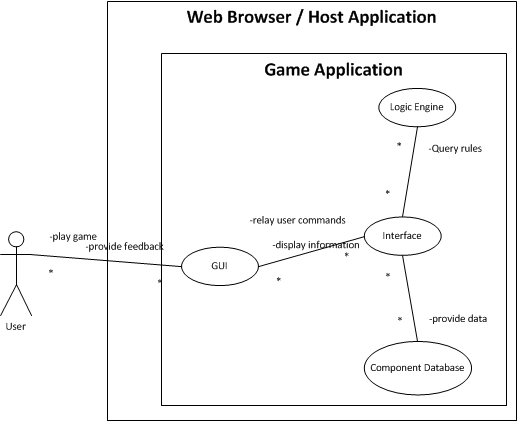
\includegraphics[width=5in]{Resources//Use Case Diagram.png}
\caption{A use-case diagram of the interactions between the sub programs.}
\label{fig:UseCaseDiagram}
\end{figure}

\subsection{Technical Overview\textcolor{red}{[FROM PRESENTATION]}}
\label{sec:Methodology:TechnicalOverview}
\subsubsection{The Component Database\textcolor{red}[FROM PRESENTATION]}
\label{sec:Methodology:TechnicalOverview:TheComponentDatabase}
This is a repository of all elements that can feasibly have an affect 
on the operation of the data centre. Examples include:

\begin{itemize}
\item Cooling systems
\item CPUs
\item Data traffic management algorithms
\item Operating times
\item Average ambient temperatures
\end{itemize}

For each of these, attributes are included, such as power
Consumption (which would be added to the overall power
consumption for the whole data-centre), purchasing cost, ideal operating 
temperature etc.

The Component Database is intended to be extensible, so that 
new technologies can be added As they become available.

Initially, an object oriented approach to the development of the database was taken
The justification of this approch is as follows:

\begin{itemize}

\item Generic classes can be used, which can be defined as being specific variations
 dependant on input parameters An example of this could be the considered to be the various
types of air conditioning system defined in section \ref{sec:ACriticalReviewOfReleventScientificAndEngineeringLiturature:StudiesIntoTheEnvironmentalEffectsAndEnergyEffiencyOfDataCenters:TheDifferentTypesOfAirConditioningEquipmentForITEnvironments}
\cite{TonyEvansTheDifferentTypesOfAirConditioningEquipmentForITEnvironmentsWhitePaper};

\item A switch-case construct could be used to define parameters supplied to an ``air conditioning system"
object at its construction, such as the devices spacial footprint, location within the room and a number 
used to define whether it is an air cooled system, a glycol cooled system, or another.

\end{itemize}

\subsubsection{Isolated testing of the Component Database}

\subsubsection{The Logic Engine\textcolor{red}{[FROM PRESENTATION]}}
\label{sec:Methodology:TechnicalOverview:TheLogicEngine}
It Will be written as a knowledge base, prototyped in a logical programming language such as Prolog or Simulink, before being written in a way that it can be used by the program interface.

Queries will consist of an entity in the Component Database being checked against the list of predicates in the Logic Engine's knowledge base. 

For example, if the user chooses a component, $A$, that has a maximum operating temperature, $T_{max}$, and then the user tries to add another component, $B$ which will raise the ambient temperature, $T_{amb}$ of the data centre above $T{max}$ , then the logic engine will prevent the Program Interface from allowing the user to add $B$.

%\begin{equation}
%\begin{split}
%&P_1 \models A \Rightarrow T_{max} \\
%&P_2 \models B \Rightarrow T_{amb} > T_{max} \\
%&C \models A \and \neg B \Rightarrow T_{amb} < %T_{max} \\
%\end{split}
%\end{equation}

\begin{equation}
\begin{split}
&P_1 \equiv A \Rightarrow T_{max} \\
&P_2 \equiv B \Rightarrow T_{amb} > T_{max} \\
&C \equiv A \land \neg B \Rightarrow T_{amb} < T_{max}
\end{split}
\end{equation}


The testing phase of this element will consist of querying a series of predicates in the knowledge base against dummy data. Once the Logic Engine works to a satisfactory extent, it will be integrated into the Testing Interface and tested against data in the Component Database.

The Logic Engine is intended to be extensible, so that if new principles are discovered that apply, they can be included.

\subsubsection{Isolated testing of the Logic Engine}

\subsubsection{The Program Interface\textcolor{red}{[FROM PRESENTATION]}}
\label{sec:Methodology:TechnicalOverview:TheProgramInterface}
This serves as the interface allowing the user to communicate with 
the program via the GUI, and for the program to query information on 
user selected components
against the logic engine.

It's development life-cycle will be in two stages:

\begin{enumerate}

\item The aforementioned “Testing Interface” will be developed in order to test the compatibility 
of the Component Database and the Logic Engine. As a test program, its input and output 
will primarily be through the command line.

\item The Testing interface will be further developed into the Program Interface by adding the
capacity for it to relay information between the other sub programs and the GUI.

\end{enumerate} 

The Program Interface will be written in JavaScript, allowing integration into a web page coded in HTML5 and CSS.

\subsubsection{Isolated testing of the Program Interface}

\subsubsection{The GUI\textcolor{red}{[FROM PRESENTATION]}}
\label{sec:Methodology:TechnicalOverview:TheGUI}
The GUI will be programmed to communicate with the program interface on the programming interface's terms. This allows multiple developments of the GUI, testing whether 2D or 3D GUIs work best with the game.

\begin{figure}[H]
\centering
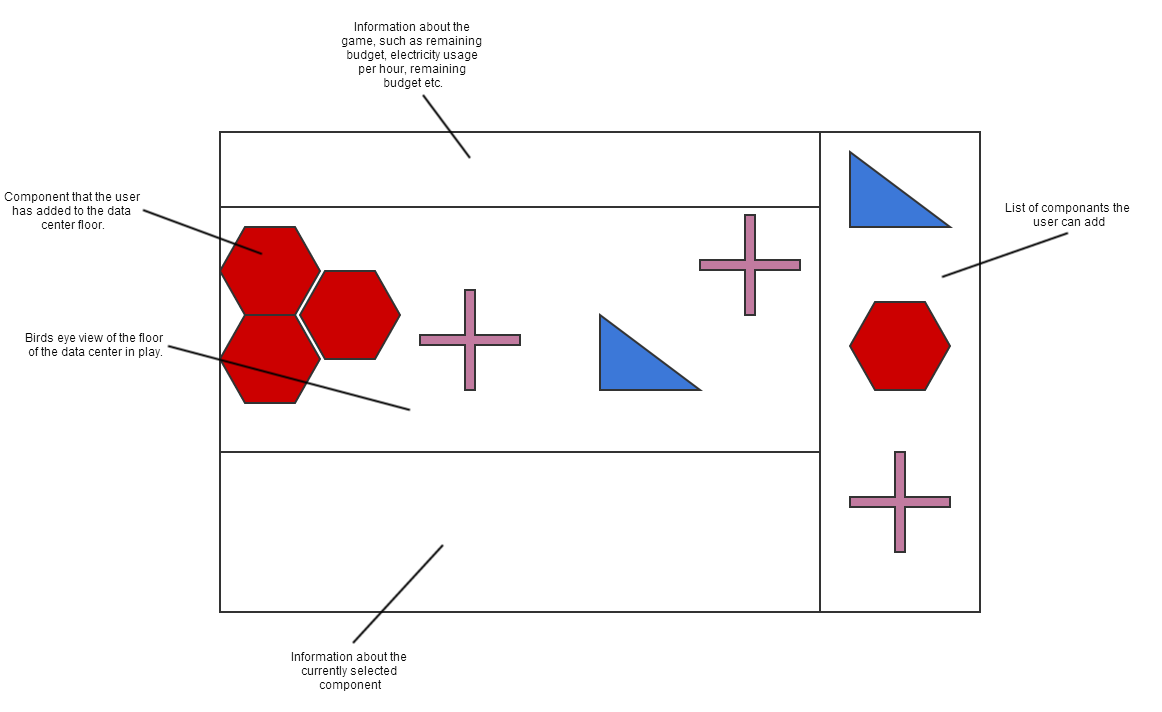
\includegraphics[width=7.25in]{Resources//GUI Mock up.png}
\caption{A mock up example of a potential GUI design, showing a top-down view of the \gls{data centre} floor, allowing users to place components from a list on the right hand side of the screen, with information about the component in the bottom pane, and general game information in the top pane.}
\label{fig:GUIMockUp}
\end{figure}

\subsubsection{Test Cycle One}
\label{sec:DevelopmentOfTheComponentDatabaseAndTheLogicEngineApplicationComponents:TestingOfTheComponentDatabaseAndTheLogicEngineViaTheTestInterface:TestCycleOne}

The first issue found was that...

This was corrected by performing the following actions:
\begin{itemize}
\item
\item
\item
\end{itemize}

The second issue found was that...

This was corrected by performing the following actions:
\begin{itemize}
\item
\item
\item
\end{itemize}

\section{Development of an Interface between the Component-Database and the Logic-Engine, and Development of a GUI}
\label{sec:DevelopmentOfAnInterfaceBetweenTheComponentDatabaseAndTheLogicEngineAndDevelopmentOfAGUI}

\subsection{Interface Development}
\label{sec:DevelopmentOfAnInterfaceBetweenTheComponentDatabaseAndTheLogicEngineAndDevelopmentOfAGUI:InterfaceDevelopment}
\textcolor{red}{The interface will be developed from the Test-Interface (section \ref{sec:DevelopmentOfTheComponentDatabaseAndTheLogicEngineApplicationComponents:TheTestInterface}). As such, this section may become obsolete and be removed.}

\subsection{The GUI}
\label{sec:DevelopmentOfAnInterfaceBetweenTheComponentDatabaseAndTheLogicEngineAndDevelopmentOfAGUI:TheGUI}
\textcolor{red}{Chronicling of the development of the GUI}

\subsection{Integration}
\label{sec:DevelopmentOfAnInterfaceBetweenTheComponentDatabaseAndTheLogicEngineAndDevelopmentOfAGUI:Integration}
\textcolor{red}{Integration of the all of the software components and the GUI together into a working program.}